\documentclass[12t]{csethesis}
%\usepackage{amsmath}
\usepackage[left=3cm,right=3cm,top=3cm,bottom=3cm,includeheadfoot,a4paper]{geometry}
\usepackage{pbox}
\usepackage{amsmath}%
%\usepackage{mathtools}
%\usepackage{datetime}
\usepackage{amsfonts}%
\usepackage{amssymb}%
\usepackage{graphicx}
%\usepackage[boxruled,vlined]{algorithm2e}
%\usepackage{color}
\usepackage{enumerate}
\usepackage{epstopdf}
\usepackage[table]{xcolor}        % Extra math definitions
\usepackage{graphics}       % PostScript figures
\usepackage{setspace}       % 1.5 spacing
\usepackage{multicol}
\usepackage{epsfig,color}
\usepackage{epstopdf}
\usepackage{graphicx}
\usepackage{lscape}
%\usepackage{epsfig}
\usepackage{enumerate}
\usepackage{algorithm}
\usepackage{algorithmic}
% \usepackage{fixltx2e}
\usepackage{tikz}
\usepackage{booktabs}
%\usepackage[ruled,vlined]{algorithm2e}
\usepackage{rotating}
\usepackage{graphicx}
\usepackage{stmaryrd}
%\usepackage{caption}
%\usepackage{subcaption}
\usepackage{colortbl}
\usepackage{subfigure}
\usepackage{wrapfig}
\usepackage{multirow}
% \usepackage{fixltx2e}
\usepackage[printonlyused]{acronym}
%\documentclass{article}
\usepackage{ifthen}
\usepackage{placeins}
\usepackage{epsfig,graphicx,color,amssymb,amsmath,comment}
\usepackage{amsfonts}
\usepackage[]{graphicx}
\usepackage{array}
\usepackage{commath}
\usepackage{cite} 
%\usepackage[]{graphicx}
\usepackage{adjustbox}
\usepackage{longtable,lscape}
\usepackage{url}
\usepackage{subfigure}
\usepackage{mathtools}
% For appendix lstlisitings
%\usepackage[T1]{fontenc}
%\usepackage{textcomp}
\usepackage{listings}
%\lstset{upquote=true}
\usepackage{appendix}
%\usepackage{hyperref}

\usetikzlibrary{shapes,shadows,arrows}
\tikzstyle{startstop} = [rectangle, rounded corners, minimum width=3cm, minimum height=1cm,text centered, draw=black, fill=red!30]
\tikzstyle{io} = [trapezium, trapezium left angle=70, trapezium right angle=110, minimum width=3cm, minimum height=1cm, text centered, draw=black, fill=blue!30]
\tikzstyle{process} = [rectangle, minimum width=3cm, minimum height=1cm, text centered, text width=3cm, draw=black, fill=orange!30]
\tikzstyle{decision} = [diamond, minimum width=3cm, minimum height=1cm, text width=3cm,text centered, draw=black, fill=green!30]
\tikzstyle{arrow} = [thick,->,>=stealth]

\usepackage{epsfig}
\phdtitle = {\textsl{TarPy: A Multi Agent Platform in Python}} 
\name = {Ajitem Joshi And Shubham Sharma}
\rollno = {194101021 and 194101047}
\guide = {Prof. Shivashankar B. Nair}


\begin{document}
\begin{titlepage}
\begin{center}
\textheight 15.5in \textwidth 12.5in {\large\sf  \textbf{\the\btptitle}}\\[12ex]
{\small{\textsl{ \textbf{An M. Tech Project Report Submitted \\
in Partial Fulfillment of the Requirements \\
for the Degree of
\\[3ex]\small \bf Master of Technology}}}}\\[16ex] \emph{by} \\[2ex]
{\sf \sf \textbf{\the\name}\\
             (\the\rollno)}\\[1ex]
\emph{under the guidance of}\\[2ex]
{\sf \bf \the\guide} \\[7ex]

\vspace{1.2in}

 \begin{figure}[!h]
 \hfill
 
\psfig{file=iitglogo.eps,width=0.15\textwidth} \hfill \
 \end{figure}

{\sl \bf{to the}} \\[1ex]

{\small\bf DATA SCIENCE PROGRAMME}  \\[1ex]
{\small \bf{INDIAN INSTITUTE OF TECHNOLOGY GUWAHATI \\GUWAHATI - 781039, ASSAM}}
%\\[2ex]
%
%  {\color{red} \hrule height 0.5ex}
% \vskip 1ex
% May \the\year 
\end{center}
\end{titlepage}

%\cleardoublepage

\newpage
\thispagestyle{empty}

\begin{center}

\huge{Department of Computer Science and Engineering}\\[0.5cm]
\normalsize
\textsc{Indian Institute Of Technology, Guwahati}\\[2.0cm]

\emph{\LARGE Certificate}\\[2.5cm]
\end{center}
\normalsize This is to certify that the project work entitled ``TarPy:  A Multi Agent Platform in Python" being submitted to Department of Computer Science and Engineering, Indian Institute of Technology Guwahati by Ajitem Joshi and Shubham Sharma in partial fulfilment for the award of the degree of Masters of Technology in Computer Science and Engineering, is a bonafide work carried out by them under my supervision. To the best of my knowledge, it has not been submitted elsewhere for the award of a degree.\\[1.0cm]



\vfill


% Bottom of the page
\begin{flushright}
..........................................\\
Prof. Shivashankar B. Nair\\
Professor\\
Department of Computer Science and Engineering\\
Indian Institute of Technology Guwahati
\end{flushright}

\begin{flushleft}
Date: $20^{th}$ November 2020
\end{flushleft}
%\cleardoublepage
\newpage
\chapter*{\centering Acknowledgement}
\large We want to take this opportunity to express our gratitude towards our supervisor Prof. Shivashankar B. Nair, for allowing us to work on this project and providing us with every useful direction for the completion of this work. We would also like to give special thankfulness to Divya Kulkarni (PhD scholar) for her constant help and support throughout our MTP. We would also like to thank Suraj Pandey (PhD scholar), Menaxi Bagchi (PhD scholar), all our friends and family for their support.


\pagenumbering{roman}

\tableofcontents
\clearpage
\addcontentsline{toc}{chapter}{List of Figures}
\listoffigures
\clearpage

%========== Chapters

\typeout{}
\clearpage
\addcontentsline{toc}{chapter}{Abstract}
\newpage
\chapter*{\centering Abstract}
\textit{\quad 
Write abstract of your theisis.
}


%\cleardoublepage
\typeout{}

\pagenumbering{arabic}
\def\headrulehook{\color{black}}

\chapter{Introduction}  \label{Introduction}

\large
In the current era, almost every sector, whether it is Healthcare, Manufacturing, Transportation Services, Robotics, and many more, has products that involve some intelligence to make the process faster and more robust to meet the industry needs. Thus, a need arises to embed intelligence in Cyber-Physical Systems(CPS). In a Cyber-Physical System, Embedded devices control the physical processes.
\par

\bigbreak
In Large Scale scenarios like natural calamity or picking up hefty loads, we need a swarm of robots to accomplish the task. If many such robots work on a single task, the problem becomes even more complicated as they need to share the information among themselves. \par

\bigbreak
The Authors in the paper \cite{semwal2015tartarus} introduce Tartarus, an Open Source Multi-agent platform for integrating CPS and Robots. Tartarus is written in SWI-Prolog\cite{wielemaker_schrijvers_triska_lager_2012} and demands the user to know Prolog Language. Agents are also called Software Robots that perform some tasks on behalf of a user or an organization. Agents\cite{10.1007/3-540-45982-0_1} in a MAS can work independently or can work collectively. Agents are said to be mobile\cite{10.1007/3-540-62852-5_4} when they move from one CPS to another over a network.\par

\bigbreak
Since Tartarus is coded in SWI-Prolog, it becomes difficult to implement intelligent algorithms as the support and popularity for Prolog has declined by a considerable margin. To enhance the application's usability, it becomes crucial to allow users to write programs in other modern languages while maintaining Tartarus's core functionality. One of the most popular modern languages that are considered powerful and provide a low bar for entry into the programming domain is Python. The low bar is a consequence of more straightforward syntax and lesser lines of code. Since Python has many libraries and more extensive community support, it becomes easy to implement algorithms and fetch support.\par
\bigbreak
\begin{figure}[!ht]
    \centerline{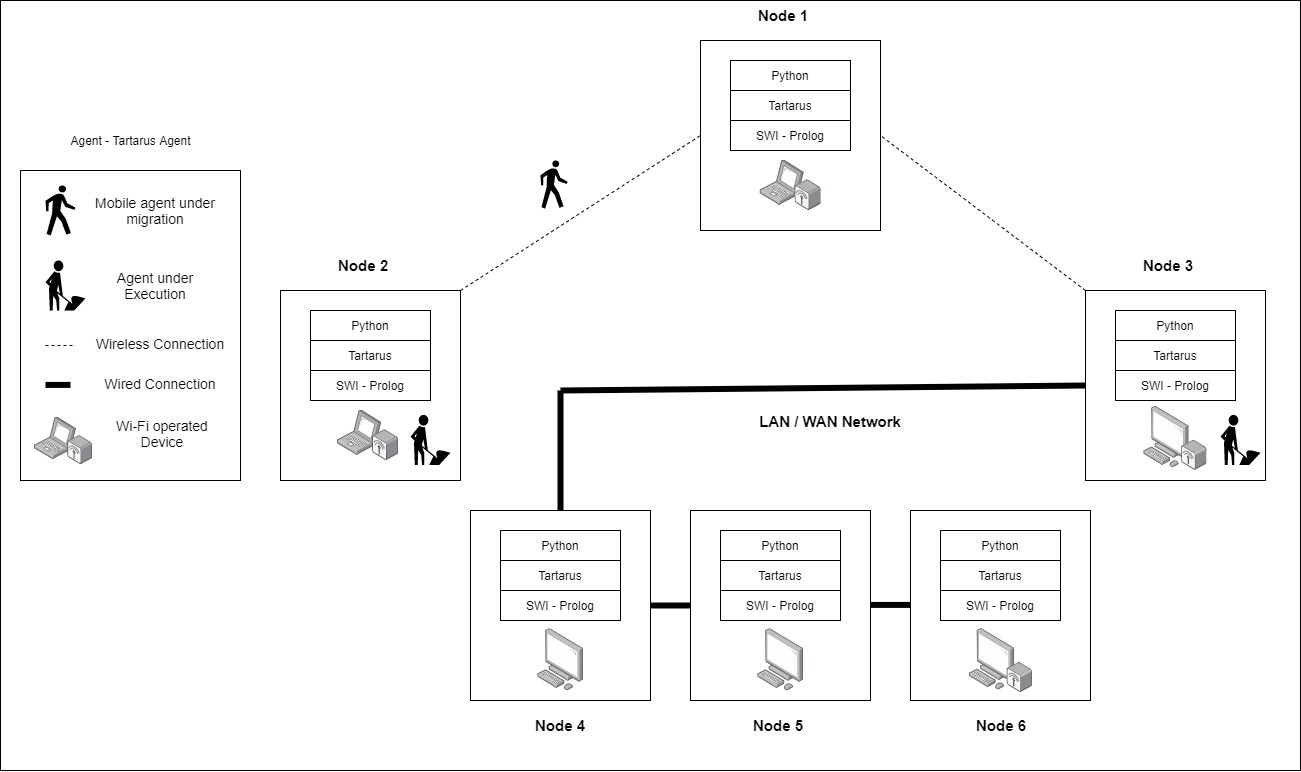
\includegraphics[width=\linewidth]{images/Nodes.jpg}}
    \caption{TarPy platform configured as a CPS}
    \label{tarpy_cps}
\end{figure}

However, one of the most revered features of Prolog is having a dynamic nature of code, which allows the code to be changed on the fly. Thus to have the best of both worlds, it is necessary to preserve the essence of Tartarus while allowing the user to code in one of the most popular programming languages.\par
\bigbreak
In this report, we present TarPy, named after Tartarus and Python. TarPy is a multi-agent platform that acts as the bridge between Tartarus and Python. TarPy implements all the Tartarus features like agent-related functionalities, multithreading, and decentralized control. TarPy works in both Linux and Windows Environment. Thereby, it can be used with various embedded controllers like Raspberry Pi, Intel Galileo.\par

\bigbreak
TarPy can be used in applications like Automating the Warehouses of the Industries wherein the Robots can communicate and distribute the work to complete in less time, Bio-inspired algorithms or genetic Algorithms can be implemented quickly to achieve decentralization and distributed learning for a common goal.\par


\bigbreak
In a multi-agent platform, various challenges need to be addressed. A situation may arise where multiple agents will visit the same node and manipulate the same data, there we need to satisfy the mutual exclusion property to maintain consistency.  Another challenge, to remove the files from the database which are no longer required. We cannot delete the data when the agent leaves the system because if the agent gets lost, then the agent's data will also get lost. While developing the TarPy many more such challenges were addressed.
\par

\bigbreak
In the Next Section, we will discuss the Platforms currently available and how TarPy is different, followed by expounding on TarPy.\par

\chapter{Related Work}


\bigbreak

\large 
Many researchers are working in domains such as Decentralization, Distributed, and Autonomous Systems. Researchers have developed various MAS platforms. Some of them include JADE\cite{10.1007/978-3-540-85058-8_15} and Aglets\cite{10.1145/295685.295882} written in Java, OSBrain and PADE\cite{pade} written in Python, and Tartarus and Typhon\cite{6524416} written in Prolog.  Apart from that, there are no Python-based MAS platforms that emphasize working with Embedded devices.
\par

\bigbreak
OSBrain\cite{OSBrain} provides the platform to implement a multi-agent and distributed system, but since it is written in Python, it does not have the dynamic code manipulation feature that Prolog has.
\par

\bigbreak
Tartarus Platform provides the decentralization and MAS with dynamic code manipulation, but Python libraries have no support.
\par

\bigbreak
All the works are done either in Java, Python or Prolog, but no platform uses multiple language features. Herein, TarPy does that and gives an edge over other available platforms.
\par

\chapter{Description and Work Done}

As mentioned in chapter \ref{Introduction}, TarPy is a multi-agent platform that acts as the bridge between Tartarus and Python. Tartarus has it's core components written in SWI-Prolog, and the benefit of changing code on the fly, thus providing a dynamic nature to the code, is not available in modern programming languages. To preserve this critical aspect of Tartarus, SWI-Prolog must be the software's core language of operations. However, since we need to ease the syntax, statistically, the most suitable language is Python. Thus, the entire package is Python at the user's end and SWI-Prolog at the agent's end.

\section{Components}
There are many components present in files that may not be independent of each other in the interaction. Typically, we require specific files to be present in order to perform our required tasks. The following section would describe various typical components for our interaction. Note that the files can be more as per use case and need not have the same name as described in the subsections.

\subsection{Tartarus Prolog Platform}
First and foremost, we require the Tartarus platform file, which is written originally in Prolog. This file contains all the Tartarus predicates for our multi-agent platform. Thus, this file would act as a base file and function at the core of the entire Python - SWI-Prolog interaction system.

\subsection{PySwip}
 We need a way to execute Prolog queries via Python. A Python library called PySwip fulfills this requirement. PySwip is a Python - SWI-Prolog bridge enabling to query SWI-Prolog in Python programs. It features an (incomplete) SWI-Prolog foreign language interface, a utility class that makes it easy querying with Prolog, and a Pythonic interface. Once PySwip is imported into Python, access the Prolog module, and assign it to a Python object. The query object would make all the further queries to Prolog.

\subsection{Tartarus Python Wrapper}
Once we have a way to communicate and query Prolog via Python, we now focus on how this can be utilized for our purpose. Tartarus is present in a Prolog file. However, we aim to have Python constructs which we can use for our Python platforms running over Tartarus. Thus, we create a Python file called \textit{`Tartarus.py'} that contains functions that query the appropriate Prolog predicates by passing the necessary parameters.

\subsection{Python Handler}
Another one of Tartarus' prominent features is the mobility of agents. Agents can move from one platform to another, unlike other software that communicates information via message passing or other means. Tartarus agents, along with their mobility, can also carry information with them in the form of payloads, which are nothing but Prolog predicates.
\par For an agent, it is essential to define its behavior and goals. Thus, we add a handler along with the agent, which takes care of the requirement. However, the agent understands the handler written in Prolog, but the developer can define the handler more conveniently in Python. Thus, the user is supposed to write a handler file in Python. This handler file written in Python is added as a payload to the mobile agent via a function \textit{`add handler()'} defined in our \textit{`Tartarus.py'} file.

\subsection{Prolog Handler} \label{Prolog Handler}
Although the user in Python well defines the agent handler, it is inevitable to have a handler in Prolog, which would work at the core of agent control. The Prolog handler typically performs the following tasks:
\begin{itemize}
    \item Retrieving the Python handler and agent database from the payload.
    \item Writing the agent Python handler and database to appropriate files.
    \item Execute the Python handler as a process.
    \item Retrieve the modified agent database information into the agent payload.
    \item Delete the agent Python files written by Prolog handler.
    \item Perform any additional specified actions.
\end{itemize}

\subsection{Temporary Agent Files}
As mentioned in \ref{Prolog Handler}, the typical Prolog handler writes the agent Python handler and Database into appropriate files. Technically, these files are strings attached as payloads to the agent in the form of predicates. Since the file names need to be unique to every agent and decided by the Prolog handler, the typical file syntax followed for Naming these files are ``agentname\_\{TYPE\}.py" where agentname would be replaced by the name of the agent and TYPE can be anything from the set \{Database, handler\_Rec, ConvertData\_to\_string\}. The purposes of these files are as follows:
\begin{itemize}
    \item \textbf{agentname\_handler\_Rec.py} file is used to write the Python handler written by the user. Since handler is Python, to execute the information and make changes in the database, it is necessary to make a process to execute Python handler.
    \item \textbf{agentname\_Database.py} file stores all the relevant data about the agent.
    \item \textbf{agentname\_ConvertData\_to\_string.py} file is used to update the Database present in agent's payload predicate.
\end{itemize}

\section{Working}
\begin{figure}[!ht]
    \centerline{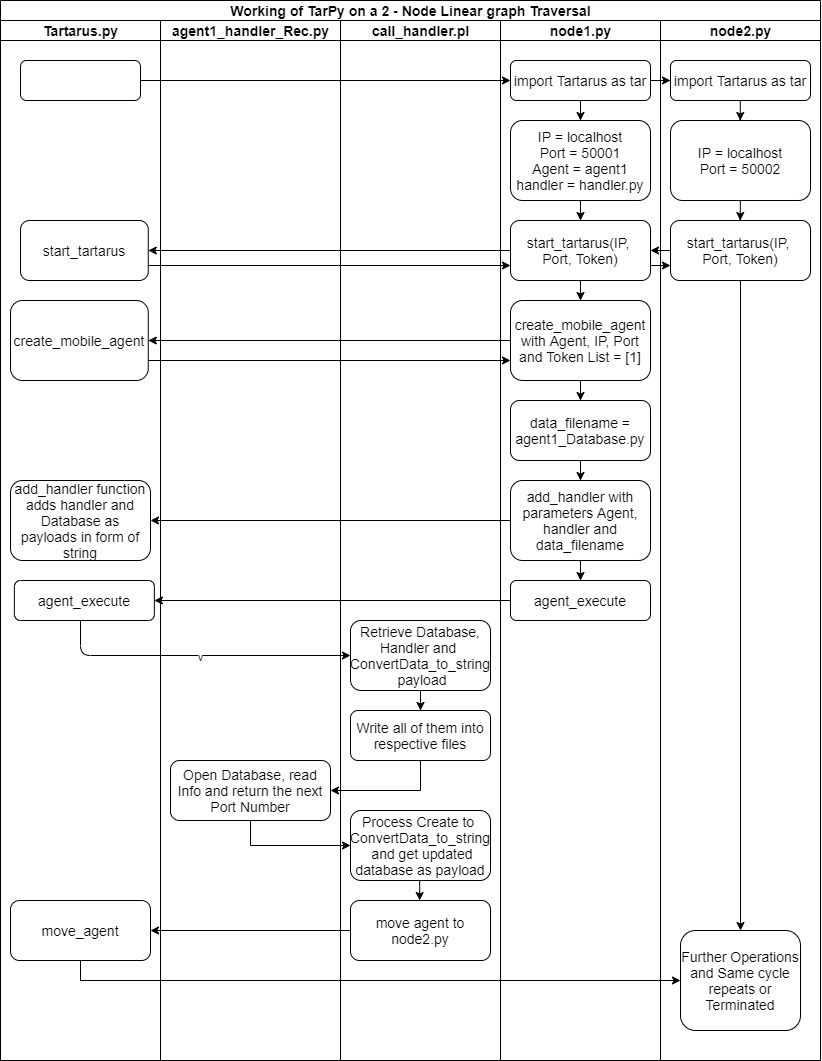
\includegraphics[width=\linewidth]{images/Working.jpg}}
    \caption{Working of TarPy for a 2 - Node Traversal}
    \label{working}
\end{figure}

Figure \ref{working} describes the working and interrelation of various components for a 2 - node traversal. \textit{node1.py} and \textit{node2.py} are the two node configuration files that execute different process instances on the same machine or another device. \textit{Tartarus.py} and \textit{platform.pl} (not shown in the figure) are present on every node. \text{handler.py} and \textit{agent1\_handler\_Rec.py} are the same programs, except that \textit{handler.py} is added as the initial payload while \textit{agent1\_handler\_Rec.py} is created by \textit{call\_handler.pl} for agent1. Thus \textit{handler.py} is not shown in the figure. The two temporary agent files, \textit{agent1\_Database.py} and \textit{agent1\_ConvertData\_to\_string.py}, are also created; however, their interaction is limited to \textit{agent1\_handler\_Rec.py}. Thus, these files are also not shown in the interaction.
\par Thus, the working of TarPy in this scenario can be described as follows:
\begin{enumerate}
    \item \textit{Tartarus.py} is imported into Python programs as `tar' in \textit{node1.py} and \textit{node2.py} 
    \item \textit{node1.py} decides IP as ``localhost" and Port as 50001 and \textit{node2.py} decide the same IP and Port as 50002.
    \item Both the nodes start the Tartarus instances by calling \textit{tar.start\_tartarus(IP, Port, 1)}, where 1 is a token for the platforms. It is necessary that node2 starts before node1 sends an agent.
\item node1 creates agent with name as agent1 on the same platform with the Token list containing 1 .
\item agent1 is expected to receive \textit{agent1\_Database.py} as a Database file stored in the \textit{`data\_filename'} variable. Since it is the initial Database before processing, its name can be arbitrary.
\item \textit{node1.py} calls \textit{tar.add\_handler} function with arguments as agent, Python handler, and data\_filename, which are added to the agent1's payload.
\item \textit{tar.agent\_execute} is called on node1, which transfers control to \textit{call\_handler.pl}, where the agent's behavior is actually executed.
\item \textit{call\_handler.pl} retrieves the payloads of the handler, Database, and ConvertData\_to\_string and writes them on the destination as files, and executes \textit{agent1\_handler\_Rec.py} as a process. \label{loop}
\item \textit{agent1\_handler\_Rec.py} operates on \textit{agent1\_Database.py} and makes the necessary changes.
\item Control resumes back to \textit{call\_handler.py} and the new Database is written back to Prolog predicate payload by calling another process on \textit{agent1\_ConvertData\_to\_string.py} file. 
\item All the files created by \textit{call\_handler.py} are removed by it as a part of cleaning procedure.
\item \textit{call\_handler.py} now executes move\_agent which moves the agent to node2
\item agent1 repeats the procedure from step \ref{loop} until termination or an invalid condition is reached.
\end{enumerate}
%\include{chapters/experiment}
\chapter{Implementation} \label{Implementation}

\large
To test the working of TarPy, we worked on some algorithms, namely Distributed MST Algorithm, Maekawa Algorithm. We went on to implement Algorithms with increasing complexity. At first, we traversed a single agent from one node to another in a sequential manner.\par

\bigbreak
For implementing any algorithm, we first need to start the Tartarus platform in every system; only after this, the agents will move in the network. After starting the Tartarus platform, the agent can be executed, now depending on the problem or the algorithm we want to implement, the logic of the handler changes.\par

\bigbreak
For the traversal, we just maintain a variable that points to the next pointer, and whenever the agent reaches a system or a node, it increments its counter and moves to that system. and when the value becomes greater than the available port no. of the system in the network, the agent stops. Code and the demo can be found at \cite{3node}.

\bigbreak 
For the Distributed MST algorithm, the agent needs a lot more than just a variable. An agent needs to know what all nodes are already visited and need to maintain a priority queue, telling which node to visit next. The priority is decided according to the weights. When the agent starts from source, it checks all its neighbor and visits the node with minimum weight, now reaching to the destination agent checks what all the neighbor the current system has, the agent push this distances in the priority queue and then moves to the next node. When all the nodes are visited, the agent stops traversing, and like this, we get the minimum spanning tree. In this, the agent follows the Prim's algorithm's logic to calculate the MST in a distributed manner. The code and demo can be found at \cite{distmst}\par
\chapter{Future Work}

\bigbreak
Every device has its environment set up in a network. The environment can vary with different operating systems. So, having a platform that works in a network of systems with multiple environments is a game-changer. The current version of the TarPy has some constraints on working in a cross-platform environment. The agent can move from Linux to Windows environment; however, the movement of agents from Windows to Linux environment is not supported.\par

\bigbreak
The current version of TarPy is not tested with embedded OS such as Raspbian OS. Compatibility with such OS can give agents access to different sensors, actuators, GPIO, etc., connected with the embedded system. The agent can use this data to learn about its environment. Here, TarPy can then allow them to develop deep learning models on such data in a federated manner.\par


\bigbreak
The platform is tested on a couple of Algorithms like traversing in a Circular fashion, Distributed Minimum Spanning Tree Algorithm, Maekawa's Algorithm for mutual exclusion in a distributed system. There can be use cases where TarPy will need some improvement at the Prolog level. In that case, it will require some basic knowledge of Prolog to enhance the features of TarPy.\par

\chapter{Conclusions}
\bigbreak
\large
This report presents TarPy, the Multi Agent Platform developed in python which provides various USPs, it makes CPS work in a decentralised and distributed environment with the agents having on the fly programming feature. The platform uses Tartarus which gives TarPy the feature of dynamic database manipulation, as tartarus is coded in prolog. The platform helps in implementing intelligent algorithms in a distributed manner, thereby CPS can implement concepts of federated learning and much more through TarPy.\par         

\bibliographystyle{IEEEtran}
\bibliography{references}
%\end{singlespace}
\clearpage

\begin{appendices}
\chapter{Code for 3 - Node Traversal} \label{traverse}
\textbf{Code for handler.py}
\begin{lstlisting}
# import agent1_Database as db -> Added by default

# Ensure that this function is same in call_handler.pl
def next_node_port(Cur_Port):
    #Extracting the Data
    next_node = db.Queue
    visited = db.Visited
    Source = db.Source
    Base = db.Base
    
    # Updating the Data
    # Add current node to visited
    visited.append(next_node)

    # Increment next_node by 1
    next_node = next_node + 1
    
    #Writing the data in the database file.-
    # Open Database file in write mode
    with open("agent1_Database.py",``w") as f:
        # Writing data to a file 
        f.write( "\\nBase = " + repr(Base) + "\\n")
        f.write( "\\nSource = " + repr(Source) + "\\n")
        f.write( "\\nQueue = " + repr(next_node) + "\\n")
        f.write( "\\nVisited = " + repr(visited) + "\\n")

    #Returning the Port
    if next_node == 4:
        return 0
    return Base + next_node

\end{lstlisting}
\clearpage
\textbf{Code for node1.py}
\begin{lstlisting}
import Tartarus as tar

Base = 50000
IP = "localhost"
Port = 50001
Agent = "agent1"
node = Port - Base
handler_file = "handler.py"
data_filename = "Database.py"

#Include platform and start tartarus
tar.include("platform_ubuntu.pl")
tar.start_tartarus(IP, Port, 2529)

while True:
    s = input("press halt to close\n")
    if s == 'halt':
        tar.close_tartarus()
        break

    if s == 'start':
        # Agent 1 has to get the next Node port to visit
        next_node = 1
        visited = []

        # Open Database file in write mode
        # Write Info required as payload(dynamic)
        with open(data_filename, "w") as f:
            # Writing data to a file 
            f.write("\nBase = " + repr(Base) + "\n")
            f.write("\nSource = " + repr(node) + "\n")
            f.write("\nQueue = " + repr(next_node) + "\n")
            f.write("\nVisited = " + repr(visited) + "\n")
        
        # Create mobile agent
        tar.create_mobile_agent(Agent, IP, Port, [2529])

        # Add Handlers as strings
        tar.add_handler(Agent, handler_file, data_filename)

        # Execute the agent
        tar.agent_execute(Agent, IP, Port)

\end{lstlisting}
\clearpage
\textbf{Code for nodeX.py where X = [2,3]}
\begin{lstlisting}

import Tartarus as tar

Base = 50000
IP = "localhost"
# Change Port to Base + X.
# For node2, Port is defined below
Port = 50002
current_node = Port - Base

tar.include("platform_ubuntu.pl")
tar.start_tartarus(IP, Port, 2529)

while True:
    s = input("press halt to close\n")
    if s == 'halt':
        tar.close_tartarus()
        break

\end{lstlisting}
\chapter{Code for Distributed MST} \label{dmst}
\textbf{Code for handler.py}
\begin{lstlisting}
import Tartarus as tar
import Database as db

#functions 
def compare(tup):
    return tup[1]

def next_node_port(Cur_Port):

    #Extracting the Data
    graph = db.Graph
    q = db.Queue
    visited = db.Visited
    Source = db.Source
    Base = db.Base
    mst = db.mst
    cost =db.cost
    
    # Updating the Data
    flag = False
    visited.add(Source)
    for tup in graph[Source]:
            if tup[0] not in visited:
                q.append((tup[0],tup[1],Source))
        
    q.sort(key = compare)
    while len(q) > 0:
        tmp = q.pop(0)
        if tmp[0] not in visited:
            flag = True
            mst.append((tmp[0],tmp[2]))
            cost += tmp[1]
            Source = tmp[0]
            break

    #Writing the data in the database file
    
    f = open( "Database.py", "w" ) 
    f.write( "\\nBase = " + repr(Base) + "\\n") 
    f.write( "\\nSource = " + repr(Source) + "\\n")
    f.write( "\\nGraph = " + repr(graph) + "\\n")
    f.write( "\\nQueue = " + repr(q) + "\\n")
    f.write( "\\nVisited = " + repr(visited) + "\\n")
    f.write( "\\nmst = " + repr(mst) + "\\n")
    f.write( "\\ncost = " + repr(cost) + "\\n")
    f.close()
       
    #Returning the Port
    if flag:
        return Base + Source  
    return 0 

\end{lstlisting}
\clearpage
\textbf{Code for nodeX.py where X = [1, 7]}
\begin{lstlisting}
import Tartarus as tar
import Database as db

def compare(tup):
    return tup[1]

# all basic varibles for intitating Tartarus
Base = 50000
IP = "localhost"

# Change Port to Base + X.
# For node1, Port is defined below
Port = 50001


# Starting the Tartarus Platform
tar.start_tartarus(IP,Port,1)

while True:
    str = input("press halt to close\n")
    
    # On halt platform gets closed.
    if str == 'halt'
        tar.close_tartarus()
        break

    # On "start" agents finds MST
    if str == 'start':
        Source = Port - Base
        # Complete graph known
        graph = 
        {
            1: [(2,2), (3,3)],
            2: [(1,2), (3,1), (4,1), (5,4)],
            3: [(1,3), (2,1), (6,5)],
            4: [(2,1), (5,1)],
            5: [(2,4), (4,1), (6,1)],
            6: [(3,5), (5,1), (7,1)],
            7: [(6,1)]
        }
        q = []
        visited = set()
        visited.add(Source)
        mst = []
        cost = 0 
        for tup in graph[Source]:
            if tup[0] not in visited:
                q.append((tup[0],tup[1],Source))
        
        # List is taken up as it tells which will be the min
        # cost tells the current overall cost of the mst
        
        q.sort(key = compare)
        while True:
            tmp = q.pop(0)
            if tmp[0] not in visited:
                mst.append((tmp[0],tmp[2]))
                cost += tmp[1]
                Source = tmp[0]
                break
        
        print("Queue is: ",q, 
        "\nVisited list: ", visited,
        "\nSource: ", Source)
        
        Agent = "groot"
        handler_file = "handler.py"
        Data_file = "Database.py"

        #Useful data in Database
        f = open( "Database.py", "w" )    
        f.write( "\nBase = " + repr(Base) + "\n")  
        f.write( "\nSource = " + repr(Source) + "\n")
        f.write( "\nGraph = " + repr(graph) + "\n")
        f.write( "\nQueue = " + repr(q) + "\n")
        f.write( "\nVisited = " + repr(visited) + "\n")
        f.write( "\nmst = " + repr(mst) + "\n")
        f.write( "\ncost = " + repr(cost) + "\n")
        f.close()

        #Agent movement
        tar.create_mobile_agent(Agent,IP,Port,[1])
        
        tar.add_handler(Agent, handler_file, Data_file)
        
        tar.move_agent(Agent,IP,Base+Source)

\end{lstlisting}
\clearpage
\end{appendices}
\end{document}
